\section{Experiments}

\subsection{Data and evaluation}
We study reconnection on PersonPath22 \cite{shuai2022personpath22}, using
its native manual keyframes and the publisher's FCOS person detections
trained on CrowdHuman, aligned frame by frame with the annotated sources.
The observation grid is nominally 5~Hz. Of the 236 public clips we assign
16 publisher-hosted training assets to development, 91 to calibration, and
hold out 74 publisher-hosted official test assets; the 55 clips carrying
external source mappings stay out of this protocol. Detector input,
matching rules and evaluation sequences are identical for every tracker
variant.

The setting is deliberately detection-only. No re-identification network
is trained and no gallery is stored: the gate must decide from geometry,
detector confidence and association margins alone. Appearance
re-identification, as in the ReID variant of BoT-SORT
\cite{aharon2022botsort}, carries an orthogonal and often stronger signal
and is the natural next comparison rather than a component of this one.

To measure detector-gap recovery, we first matched detection boxes and
ground-truth persons one to one at IoU $\geq 0.50$. For each ground-truth
identity, a gap consisted of one to five intervening annotated keyframes
with no matched detection. We counted a recovery if the track identifier
at the first returned detection matched its identifier before the gap. We
used the same ground-truth/detector gap list for all policies and included
cases without an emitted pre-gap identity in the denominator.

We also audited the tracker's reactivation actions separately from gap
recovery. A reactivation was correct if the specified one-to-one matching
assigned its previous emitted track and its new detector box to the same
annotated person; otherwise it was counted as wrong or unverifiable,
except where an unmatched endpoint overlapped an annotated ignore region
by more than half its own box area. Ignored actions are reported
separately. The audit runs after tracking, so the gate itself never sees
an annotation. Overall metrics were HOTA, AssA, IDF1 and ID switches,
computed with TrackEval on the native keyframe grid
\cite{luiten2021hota}, with PersonPath22's distractor and crowd treatment.

\subsection{Comparison and model fitting}
We replayed ByteTrack \cite{zhang2022bytetrack} and a motion-only BoT-SORT
configuration \cite{aharon2022botsort}, each from frame one, with the gate
deciding on every native old-ID reactivation before the tracker updated
its state. We compared the unrestricted tracker, a source cap alone, a
threshold on the native association cost, a threshold on the nearest
competitor margin, an additive linear score, the interaction score, and
the interaction score with the within-source ranking term. Capped policies
admit at most 12 actions per source, and ignored admissions count against
the cap as well. Scores were fit on the development sources for 200
Adam updates (learning rate 0.04, coefficient penalty 0.002) on a GeForce
RTX 3060 Ti. Candidate thresholds came from development score quantiles
fixed before calibration. For each score we take the operating point that
recovers the most gaps within a common empirical calibration ceiling while
keeping at least 20\% of calibration sources active, then run the selected
policies on the official test assets without tuning.

\subsection{Official split results}
The official test subset contained 9,320 keyframes and 3,155 eligible
detector gaps. At a common empirical calibration ceiling of 47.23\%, the
ByteTrack interaction gate reduced the tested incorrect or unverifiable
action proportion from 46.77\% to 35.39\% relative to the native
association threshold, and raised verified correct reactivations from 239
to 283 while using 438 evaluated admissions instead of 449. Gap recoveries
were 393 and 388. The paired source resampling interval was
$[-16.57,-6.40]$ percentage points for the failure-rate difference and
$[-0.33,0.67]$ for gap recovery (10,000 replicates). The interaction score
also reduced the failure proportion against the cap-only and linear
controls at this ceiling.

At the 20\% calibration ceiling both ByteTrack scores recovered 383 gaps,
with observed failure proportions of 21.24\% for the interaction score and
21.15\% for the linear score. On motion-only BoT-SORT the interaction
score recovered 334 gaps against 327 for the linear score, with 16.19\%
versus 18.31\% checked failures. The paired intervals were $[0.05,0.48]$
percentage points for gap recovery and $[-4.94,0.75]$ for the failure
proportion. At the relaxed BoT-SORT ceiling of 42.15\% the linear score
had the lower observed failure, 25.19\% against 37.28\%. The added
pairwise ranking loss produced no consistent benefit.

\begin{figure*}[t]
\centering
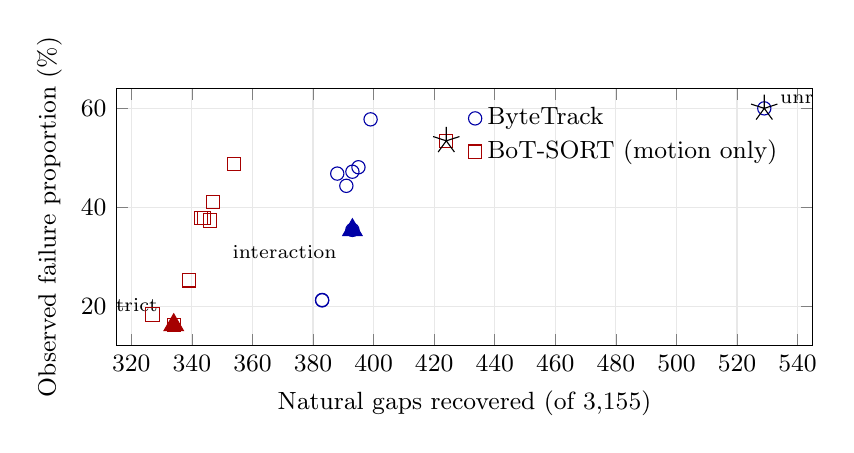
\begin{tikzpicture}
\begin{axis}[
    width=0.86\textwidth,
    height=0.40\textwidth,
    xlabel={Natural gaps recovered (of 3,155)},
    ylabel={Observed failure proportion (\%)},
    xmin=315, xmax=545,
    ymin=12, ymax=64,
    grid=major,
    grid style={gray!18},
    legend pos=north east,
    legend cell align=left,
    legend style={draw=none, fill=none, font=\small},
    tick label style={font=\small},
    label style={font=\small},
    mark size=2.4pt,
]
\addplot[only marks, mark=o, mark options={solid}, color=blue!65!black,
         forget plot] coordinates {
    (529,59.95) (399,57.73) (388,46.77) (391,44.30) (395,48.05)
    (393,35.39) (393,47.15) (383,21.15) (383,21.24)
};
\addlegendimage{only marks, mark=o, color=blue!65!black}
\addlegendentry{ByteTrack}
\addplot[only marks, mark=square, mark options={solid}, color=red!65!black,
         forget plot] coordinates {
    (424,53.39) (354,48.69) (343,37.76) (347,41.02) (339,25.19)
    (346,37.28) (344,37.78) (327,18.31) (334,16.19)
};
\addlegendimage{only marks, mark=square, color=red!65!black}
\addlegendentry{BoT-SORT (motion only)}
\addplot[only marks, mark=star, mark size=5pt, color=black] coordinates {(529,59.95)};
\addplot[only marks, mark=star, mark size=5pt, color=black] coordinates {(424,53.39)};
\addplot[only marks, mark=triangle*, mark size=4pt, color=blue!65!black] coordinates {(393,35.39)};
\addplot[only marks, mark=triangle*, mark size=4pt, color=red!65!black] coordinates {(334,16.19)};
\node[font=\scriptsize, anchor=south west] at (axis cs:531,59.0) {unrestricted};
\node[font=\scriptsize, anchor=north east] at (axis cs:391,34.2) {interaction};
\node[font=\scriptsize, anchor=south east] at (axis cs:332,16.9) {strict};
\end{axis}
\end{tikzpicture}
\caption{Every evaluated policy on the official PersonPath22 test subset,
plotted by the number of natural gaps it recovers and the observed
proportion of failed evaluated reactivations. Stars mark the unconstrained
trackers, triangles the relaxed interaction gate, and the lower-left
cluster the strict ceilings. Policies to the right of a given point recover
more gaps; policies below it fail less often. The frontier runs from the
strict ceilings at the lower left to the unconstrained tracker at the upper
right, so no single policy is best on both axes.}
\label{fig:tradeoff}
\end{figure*}


\begin{table*}[t]
\centering
\small
\caption{PersonPath22 native-keyframe official-test subset. Gap recovery
uses the same 3,155 gaps for every policy. Admits and fails exclude
ignored actions. HOTA, AssA and IDF1 are on a 0--100 scale; IDSW is a
count; Risk is the observed failure proportion. The cap-only gate applies
the same source cap. Rows without a strict marker use the relaxed
calibration ceiling. Section~\ref{sec:matched} re-selects thresholds under
a matched-acceptance rule, so its counts differ from these.}
\label{tab:reconnection-main}
\begin{tabular}{llrrrrrrrr}
\hline
Tracker & Reactivation policy & Gaps kept & Admits & Fails & Risk (\%) & HOTA & AssA & IDF1 & IDSW \\
\hline
OC-SORT & External reference & 174 & -- & -- & -- & 41.83 & 41.22 & 52.15 & 3790 \\
\hline
ByteTrack & Unrestricted & 529 & 2589 & 1552 & 59.95 & 46.64 & 42.33 & 56.73 & 6662 \\
 & Cap only & 399 & 537 & 310 & 57.73 & 44.69 & 39.32 & 52.94 & 7129 \\
 & Native cost & 388 & 449 & 210 & 46.77 & 44.76 & 39.41 & 53.16 & 7104 \\
 & Nearest margin & 391 & 456 & 202 & 44.30 & 44.84 & 39.57 & 53.14 & 7132 \\
 & Linear & 395 & 514 & 247 & 48.05 & 44.90 & 39.63 & 53.38 & 7131 \\
 & Interaction & 393 & 438 & 155 & 35.39 & 44.99 & 39.81 & 53.38 & 7022 \\
 & Interaction + ranking & 393 & 509 & 240 & 47.15 & 44.91 & 39.69 & 53.34 & 7131 \\
 & Linear (strict) & 383 & 331 & 70 & 21.15 & 44.87 & 39.63 & 53.25 & 7120 \\
 & Interaction (strict) & 383 & 339 & 72 & 21.24 & 44.87 & 39.63 & 53.23 & 7116 \\
\hline
BoT-SORT & Unrestricted & 424 & 1858 & 992 & 53.39 & 46.84 & 43.78 & 56.57 & 5909 \\
(motion only) & Cap only & 354 & 495 & 241 & 48.69 & 45.04 & 40.71 & 53.03 & 6616 \\
 & Native cost & 343 & 392 & 148 & 37.76 & 44.99 & 40.67 & 52.98 & 6656 \\
 & Nearest margin & 347 & 451 & 185 & 41.02 & 45.10 & 40.83 & 53.07 & 6654 \\
 & Linear & 339 & 397 & 100 & 25.19 & 45.20 & 40.99 & 53.29 & 6603 \\
 & Interaction & 346 & 448 & 167 & 37.28 & 45.14 & 40.88 & 53.20 & 6566 \\
 & Interaction + ranking & 344 & 450 & 170 & 37.78 & 45.14 & 40.87 & 53.16 & 6611 \\
 & Linear (strict) & 327 & 284 & 52 & 18.31 & 45.05 & 40.83 & 53.05 & 6628 \\
 & Interaction (strict) & 334 & 278 & 45 & 16.19 & 45.06 & 40.85 & 53.02 & 6626 \\
\hline
\end{tabular}
\end{table*}

The unrestricted trackers retain more natural gaps and higher overall
HOTA (Table~\ref{tab:reconnection-main}). Relative to unrestricted
ByteTrack, the relaxed interaction gate removes 1,397 evaluated failures
and 136 natural gaps, and HOTA falls by 1.65 points. That is the price of
selective admission, and we state it as a price rather than argue it away:
the gate buys decision reliability, not a better tracker. OC-SORT
\cite{cao2023ocsort} appears as an overall tracking reference whose output
supports the same gap evaluation, although its internal reactivation
mechanism follows a different protocol.

\subsection{Matched acceptance}
\label{sec:matched}

Counting failures rewards silence. A gate that admits nothing has no
failures, and Table~\ref{tab:reconnection-main} compares policies that
admit anywhere from 278 to 2,589 actions, so part of its ordering reflects
admission count rather than decision quality. We remove that confound
directly: for each tracker and each cap $B\in\{6,12,24\}$ we re-select
thresholds so that the native association cost, the additive score and the
interaction score admit the same number of actions per source.

Matching is not free. The target is the calibration admission count per
source, and a method may deviate by 0.10 admissions per source or 5\% of
the target, whichever is larger. None of the 18 cells of the original
quantile grid cleared that bar, so the sweep was densified to steps of
0.01 and replayed on calibration until 17 operating points could be
locked. Seven of them
still satisfied the between-method tolerance on the test sources; the
other ten are reported as sensitivity results. In all 17, at least one
method ends further from its calibration target than the tolerance allows,
so these are comparisons between methods, not reproductions of a fixed
admission rate.

Against the native association cost the interaction score had the lower
failure proportion at all 17 points, by 8.70 to 23.00 percentage points,
with every per-comparison interval below zero. At the cap of 12 and the
high ceiling the gap is concrete: ByteTrack fails in 98 of 381 evaluated
admissions against 158 of 390, and motion-only BoT-SORT in 81 of 367
against 116 of 350, with paired intervals of $[-20.95,-8.80]$ and
$[-17.29,-5.15]$ points. Gap recovery moves by $+0.41$ $[+0.03,+0.84]$
and $+0.10$ $[-0.35,+0.60]$ points. The reliability gain therefore does
not cost recovery at this operating point, and it is not an artefact of
admitting less.

Against the additive score the picture is thinner. Two of the 17 contrasts
have an interval entirely below zero -- $-3.29$ $[-5.37,-1.10]$ at the
ByteTrack high point and $-2.57$ $[-5.05,-0.16]$ for BoT-SORT at $B=24$ --
and the remaining 15 cross zero, several with a positive point estimate
($+1.54$ $[-1.83,+4.85]$ at the ByteTrack mid point). Matching admission
counts separates the interaction score from the native cost cleanly and
from an additive model only at some operating points. We keep that
distinction instead of averaging over it.

\subsection{Where the gain comes from}
\label{sec:ablation}

Two questions decide whether the score is a contribution or a fitted
artefact: which part of $\phi$ carries the effect, and whether a published
association score does the same job more simply.

For the first we build three scores on identical development proposals,
labels and sample order. The 12-dimensional and the full 23-dimensional
scores reuse their locked weights. The 15-dimensional score keeps the 12
base features and adds three competition summaries -- the minimum margin,
the absolute difference of the margins, and the largest transformed
alternative count -- and is refitted from scratch, since truncating the
full model's weights cannot separate the two hypotheses. Fitting uses the
original settings, including an explicit ranking weight of zero. The
15-dimensional feature prefix is verified to equal the first 15 entries of
the full vector on the same proposal, and the reloaded 12- and
23-dimensional configurations reproduce their stored scores.

Table~\ref{tab:round3} gives the paired contrasts. Adding the eight product
terms to the 15-dimensional score lowers the failure proportion by 3.29
points at the ByteTrack high point, interval $[-5.82,-0.92]$. At the mid
point the difference reverses to $+1.60$ $[-1.43,+4.48]$, and all three
BoT-SORT intervals cross zero. The three competition summaries alone
produce no contrast whose interval excludes zero at any of the five
points. The effect belongs to the group of product terms as a whole, and
it is established at one operating point rather than throughout.

For the second question we port the association similarity of the published
BoostTrack tracker \cite{stanjoevic2024boosttrack} into the same role. The
host tracker assigns exactly as
before; for the proposals it has already made, we read the BoostTrack
similarity of the proposed pair from the current-frame candidates and the
host track state, then apply the same gate and the same handling of
refused detections. Detection boxes, scores, native assignments, motion
updates and later stages are untouched. A switched scoring component can
otherwise be confused with a change of input, so the port is checked
numerically first: on 1,747 development candidate matrices the ported and
the authors' function agree to a maximum absolute difference of zero
across 745,096 elements, and for motion-only BoT-SORT, whose state stores
width and height rather than height and aspect ratio, 420,620 elements
agree to zero with the covariance propagated by a first-order
approximation.

\begin{table*}[t]
\centering
\small
\caption{Interaction ablation and external score, cap of 12 admissions per
source. Each row is one paired contrast over the same 74 sources,
resampled 10,000 times (seed 362). Fails/admits counts evaluated decisions
after ignore-region removal and is not the gap-recovery denominator.
$\Delta$ is the left policy's failure proportion minus the right policy's,
in percentage points; negative favours the left policy. BoostTrack rows
compare the ported association score inside the same host.}
\label{tab:round3}
\begin{tabular}{lllrrr}
\hline
Tracker & Ceiling & Contrast & Fails/admits (L / R) & $\Delta$ (pp) & 95\% CI \\
\hline
ByteTrack & high & 23 vs 15 & 98/381 \;/\; 112/386 & $-3.29$ & $[-5.82,-0.92]$ \\
 & mid & 23 vs 15 & 69/327 \;/\; 62/318 & $+1.60$ & $[-1.43,+4.48]$ \\
 & high & 23 vs BoostTrack & 98/381 \;/\; 152/388 & $-13.45$ & $[-19.06,-8.06]$ \\
 & mid & 23 vs BoostTrack & 69/327 \;/\; 109/315 & $-13.50$ & $[-18.88,-8.40]$ \\
\hline
BoT-SORT & low & 23 vs 15 & 30/222 \;/\; 33/225 & $-1.15$ & $[-3.02,+0.46]$ \\
(motion) & mid & 23 vs 15 & 57/293 \;/\; 54/291 & $+0.90$ & $[-1.56,+3.54]$ \\
 & high & 23 vs 15 & 81/367 \;/\; 81/359 & $-0.49$ & $[-2.46,+1.40]$ \\
 & low & 23 vs BoostTrack & 30/222 \;/\; 53/214 & $-11.25$ & $[-17.32,-5.32]$ \\
 & mid & 23 vs BoostTrack & 57/293 \;/\; 83/273 & $-10.95$ & $[-18.09,-3.84]$ \\
 & high & 23 vs BoostTrack & 81/367 \;/\; 110/346 & $-9.72$ & $[-16.00,-3.66]$ \\
\hline
\end{tabular}
\end{table*}

The interaction score fails less often than the ported score in all five
contrasts, by 13.45 and 13.50 points for ByteTrack and by 9.72 to 11.25
points for BoT-SORT, with every interval below zero
(Table~\ref{tab:round3}). Recovery differs by at most 0.25 points and
every such interval crosses zero. At the ByteTrack high point HOTA reads
44.98, 44.97 and 44.78 for the interaction, 15-dimensional and BoostTrack
scores. The comparison concerns the scoring component inside a common
host; the BoostTrack tracker as a whole is a different object. One
qualification applies to the whole table: no contrast reproduces its
calibration target on both sides at test time, and the BoT-SORT low point
of 15 against 12 exceeds the between-method tolerance. Thresholds were not
re-selected in response, and the numbers are the locked ones.

\subsection{Transfer across datasets}
We transferred the PersonPath22 ByteTrack thresholds to 40 previously
unseen clips under the DanceTrack training partition, with a frozen COCO
YOLOX-X detector. The relaxed interaction gate recovered 1,506 of 8,472
gaps and failed in 199 of 462 accepted actions (43.07\%); the native-cost
gate recovered 1,500 gaps and failed in 212 of 463 (45.79\%). The
20\%-calibration interaction gate had 30.03\% evaluated failures in
DanceTrack. In a five-video exploratory BDD100K transfer, the ByteTrack
interaction gate at the stricter operating point had three failures among
eight accepted actions against 16 among 25 for unrestricted ByteTrack,
with each policy retaining five of the 121 eligible detector gaps. Under
new detectors and new acquisition conditions the absolute failure
proportions rise well above PersonPath22 levels, while the ordering
between scores persists.

\subsection{Cost and sensitivity}
We reassigned numerically equivalent duplicate detector boxes within 0.001
pixels per coordinate when their matched ground-truth identity was
unambiguous. This post hoc check changed none of the accepted or failed
action counts in the relaxed ByteTrack native-cost and interaction
comparisons, nor in the strict BoT-SORT linear and interaction
comparisons. The relaxed ByteTrack interaction gate retained annotated
identity 66 across keyframes 47--49 of \texttt{uid\_vid\_00013}, where the
native threshold missed the return; the converse occurred for identity 20
across keyframes 66--68 of \texttt{uid\_vid\_00008}.

Median association and decision-logging time was 1.60 and 1.54 ms per
keyframe for unrestricted and relaxed interaction ByteTrack, and 1.48 and
1.49 ms for unrestricted and strict interaction BoT-SORT. These timings
cover seven CPU replays of 293 development keyframes each, excluding
detector inference and evaluation. The gate is a scalar evaluation per
proposal, so its cost does not grow with the number of tracks.

\subsection{Scope}
Every analysis after Table~\ref{tab:reconnection-main} reuses the same 74
assets. The matched-acceptance points, the ablation and the external
comparison are sensitivity analyses over one set of sources, not
independent replications, and no interval accounts for the others. The
gate uses no appearance signal, which bounds the claim to detection-only
pipelines. The cap of 12 admissions per source is a design parameter: the
ordering of methods holds across the caps we locked, the absolute numbers
do not. Cross-dataset results transfer frozen thresholds and nothing else.
